\documentclass[UTF8]{ctexart}

% 插图工具
\usepackage{graphicx}
\graphicspath{{./images/}}
\usepackage{subcaption}

% 插公式
\usepackage{amsmath}

\title{给王帅的demo}
\author{雷晓悦}
\date{\today}

\begin{document}
    \maketitle
    一定要用xelatex编译!!!可以把xelatex设为第一个Recipe,Ctrl+S时就会默认用它编译。
    \section{表}
    % 可调参数 https://www.overleaf.com/learn/latex/tables
    \begin{center}
        \begin{tabular}{c r l c|c}
            \hline
            c & r & l & \& & | \\
            \hline\hline
            居中 & 居右 & 居左 & 分割单元格 & 分割线\\
            \hline
        \end{tabular}
    \end{center}

    \section{图} % 可调参数:https://www.overleaf.com/learn/latex/Inserting_Images
    
    \begin{figure}[h]
        \centering
        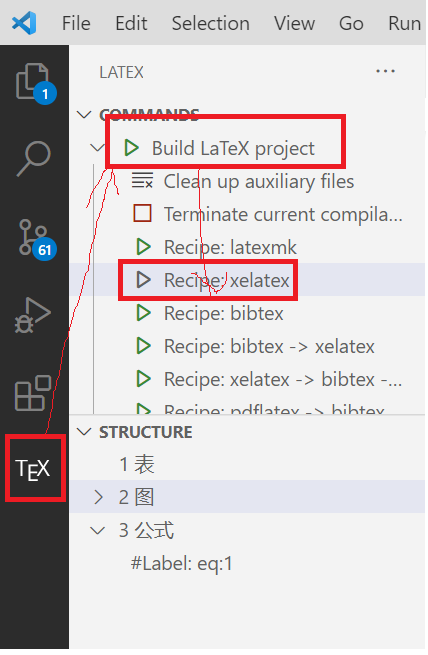
\includegraphics[width=0.3\linewidth]{xelatex_compiler.png}
        \caption{一定要用xelatex编译!}
    \end{figure}

    \begin{figure}
        \subcaptionbox{Swan\label{fig:swan}}
        {
\includegraphics[width=0.495\linewidth]{Swan.png}}
        \subcaptionbox{headtail\label{fig:headtail}}
        {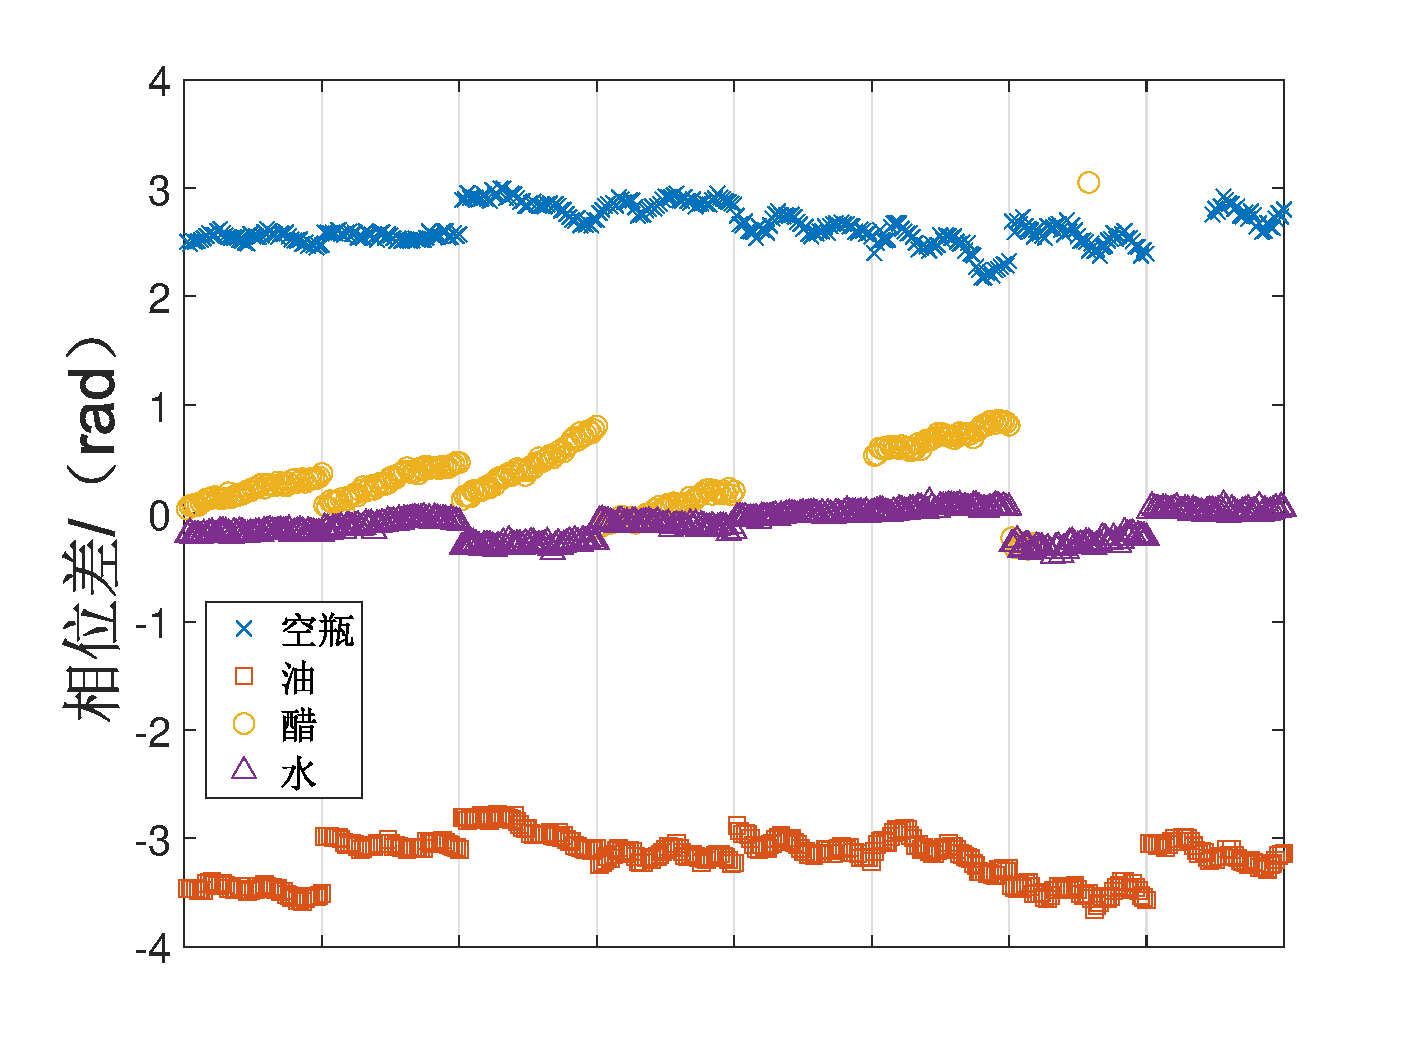
\includegraphics[width=0.495\linewidth]{headtail_phase_diff.pdf}}
    \end{figure}

    \section{公式} % More: https://www.overleaf.com/learn/latex/mathematical_expressions
    
    \begin{equation}\label{eq:1}
        a = b + c
    \end{equation}
    
    \begin{equation}
        \begin{split}
            a &= (b + c) + d \\
            &= b + (c + d)
        \end{split}
    \end{equation}

    \begin{align}
        a = b + c\\
        b = a - c\\
        c = a - b
    \end{align}
\end{document}